% Chapter Template

\chapter{Ensayos y resultados} % Main chapter title

\label{Chapter4} % Change X to a consecutive number; for referencing this chapter elsewhere, use \ref{ChapterX}


%----------------------------------------------------------------------------------------
%	SECTION 1
%----------------------------------------------------------------------------------------
En este capítulo se detallan los resultados esperados y obtenidos sobre cada prueba empleada para validar la integración del sistema y poder comprobar que el alcance funciona logrado es acorde a los esperado.
\citep{ARTICLE:1}, \citep{BOOK:1}, \citep{BOOK:2}, \citep{WEBSITE:1}.
\section{Banco de pruebas}

Todos los ensayos que se describen en este capítulo fueron efectuados utilizando el diseño físico de red que se muestra en la fig.....  Los pruebas de funcionalidad remota se realizo usando un dispositivo móvil con acceso a la red celular mediante el uso de paquete de datos de Internet.

\begin{figure}[htbp]
	\centering
	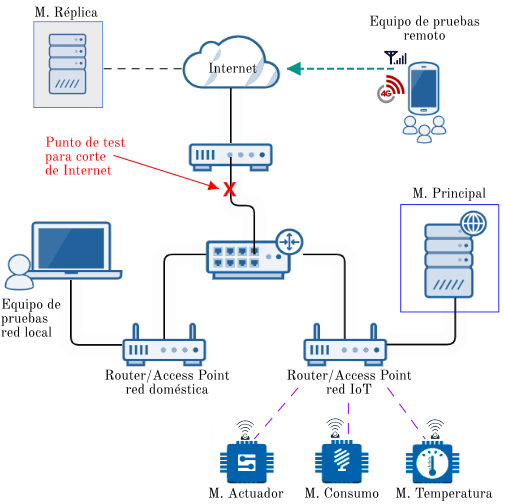
\includegraphics[width=0.91\textwidth]{./Figures/banco2.png}
	\caption{Esquema del banco de pruebas utilizado.}

	\label{fig:banco}
\end{figure}


\section{Resultados de los módulos del sistema IoT}

fotos del modulo principal.

\begin{figure}[htpb]
\centering 
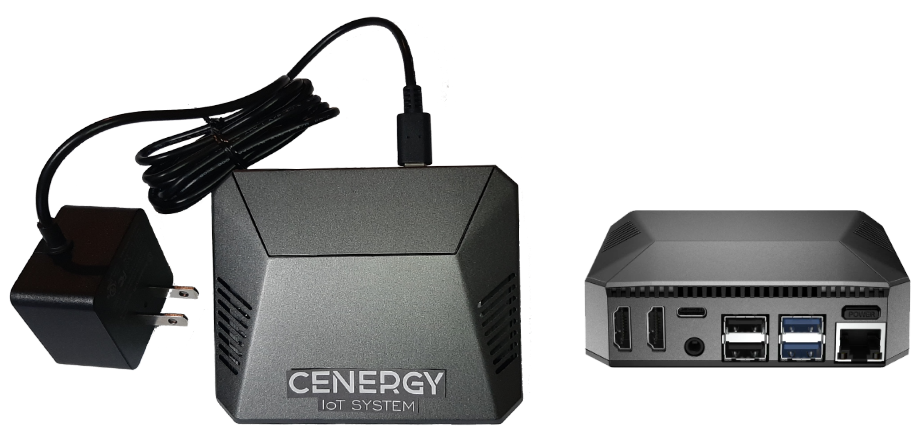
\includegraphics[width=0.95\textwidth]{./Figures/principal2.png}
\caption{Vista superior y posterior del módulo principal.}
\label{fig:modPrincipal}
\end{figure}

foto del modulo de temperatura.

\begin{figure}[htpb]
\centering 
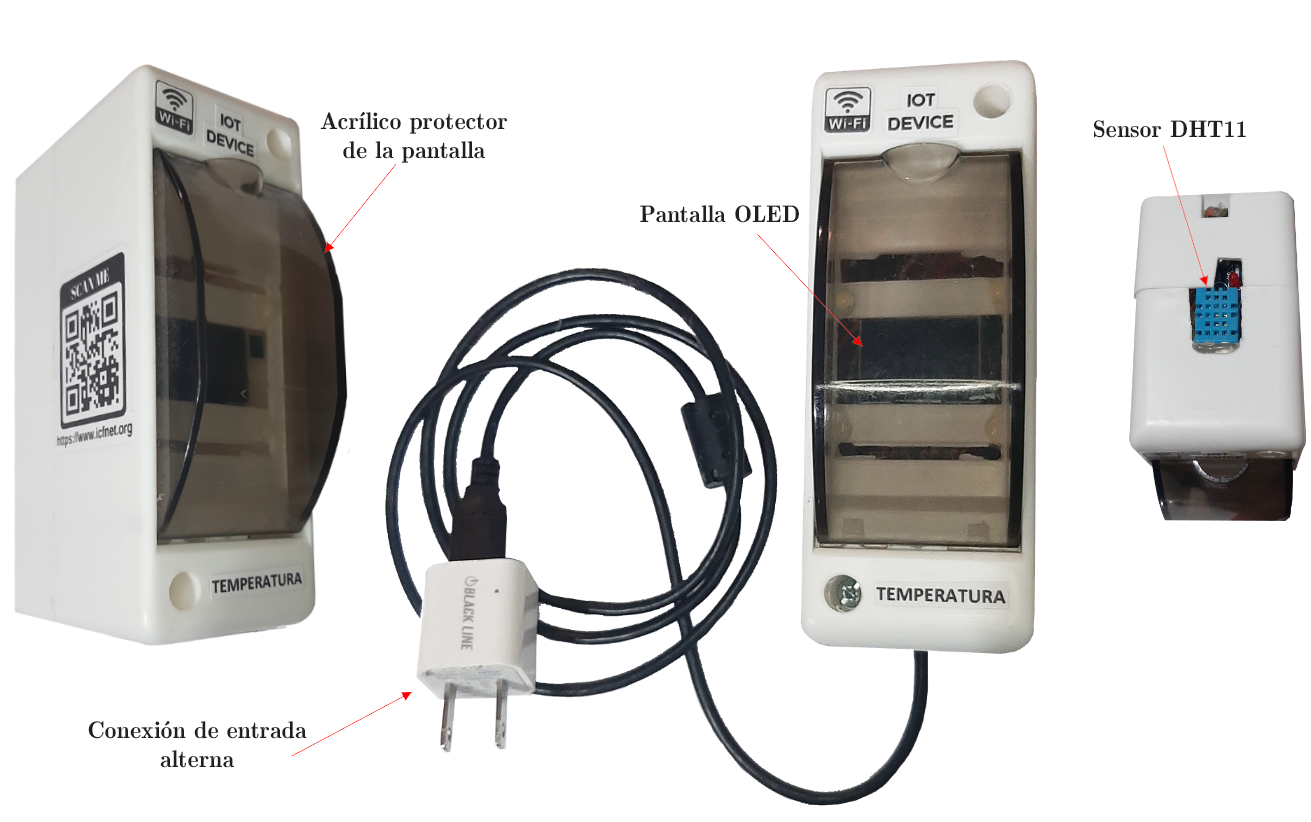
\includegraphics[width=0.9\textwidth]{./Figures/moduloTemp.png}
\caption{Vista lateral, frente y superior del módulo de temperatura.}
\label{fig:modTemp}
\end{figure}

foto del modulo actuador y consumo.

%%%%%%%%%%%%%%%%%%%%%%%%%%%%%%%%%%%%%%%%%%%%%%%%%%%

\begin{landscape} % esto es para rotar la pagina e imagen
\begin{figure}[htpb]
\centering 
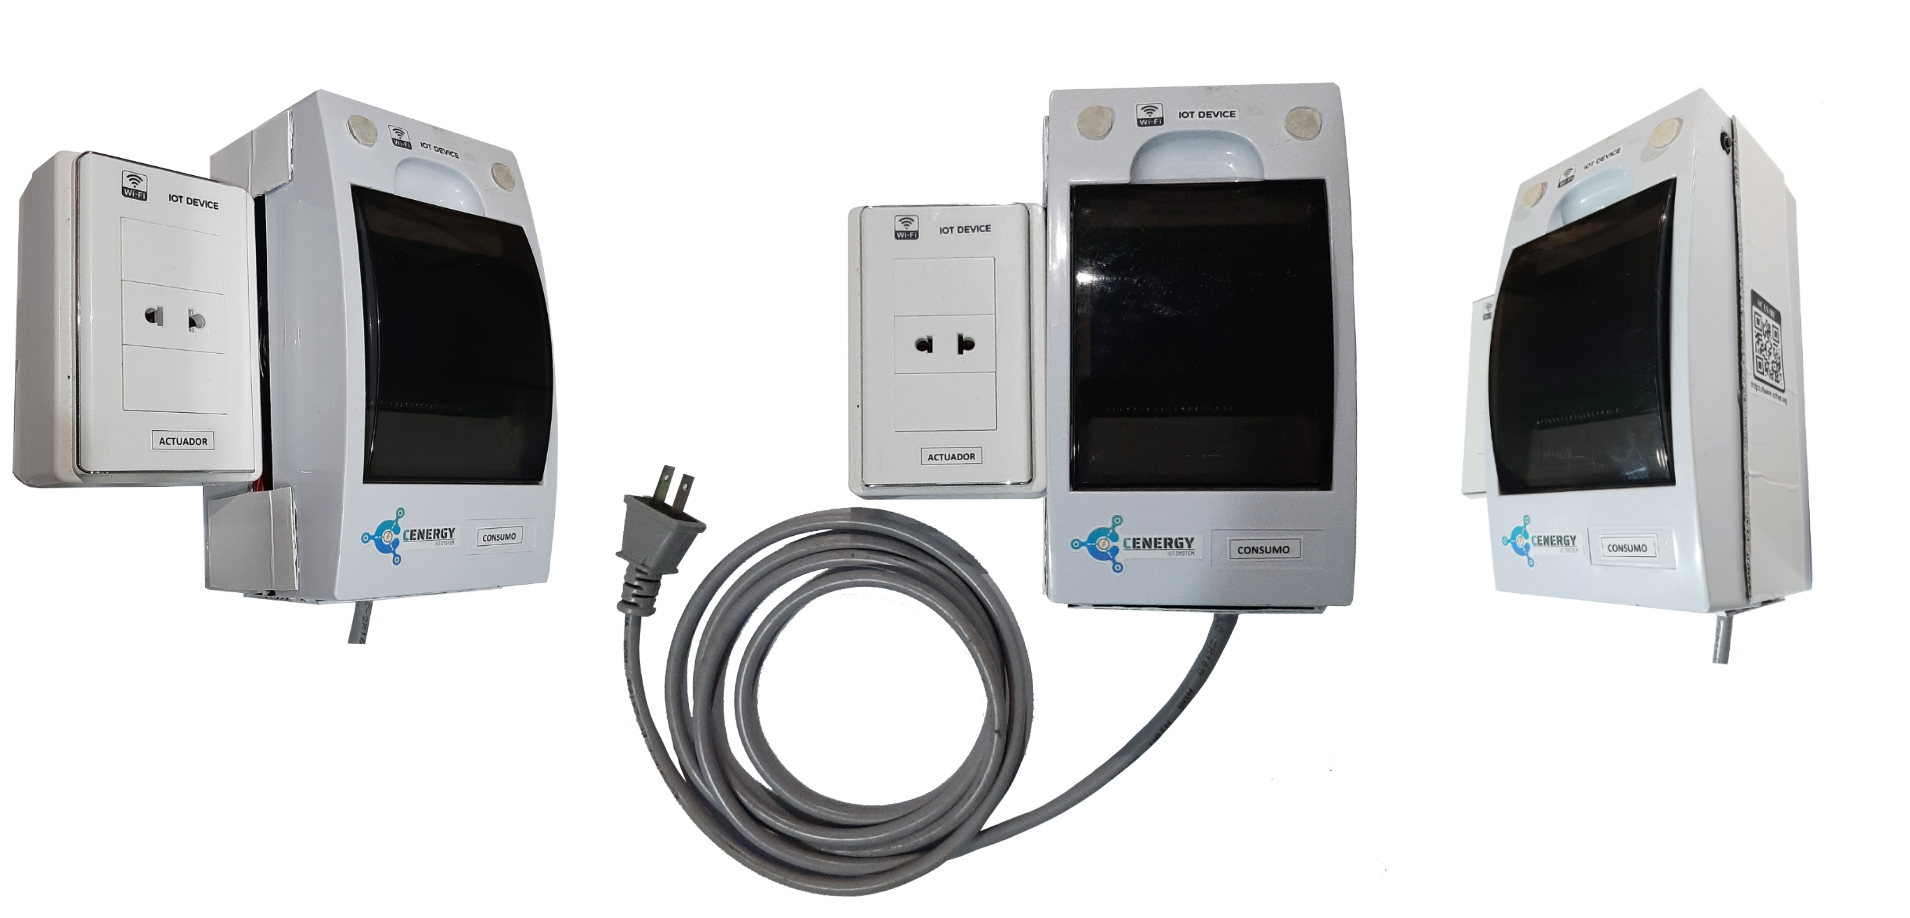
\includegraphics[width=1.8\textwidth]{./Figures/consumo2.png}
\caption{Vista frontal y lateral del módulo actuador y módulo de consumo.}
\label{fig:modConsumo2}
\end{figure}
\end{landscape} %


%%%%%%%%%%%%%%%%%%%%%%%%%%%%%%%%%%%%%%%%%%%%%%%%%%%
\section{Interfaces gráficas del sistema de monitoreo}

%%%%%%%%%%%%%%%%%%%%%%%%%%%%%%%%%%%%%%%%%%%%%%%%%%%
\begin{landscape} % esto es para rotar la pagina e imagen
\begin{figure}[htpb]
\centering 
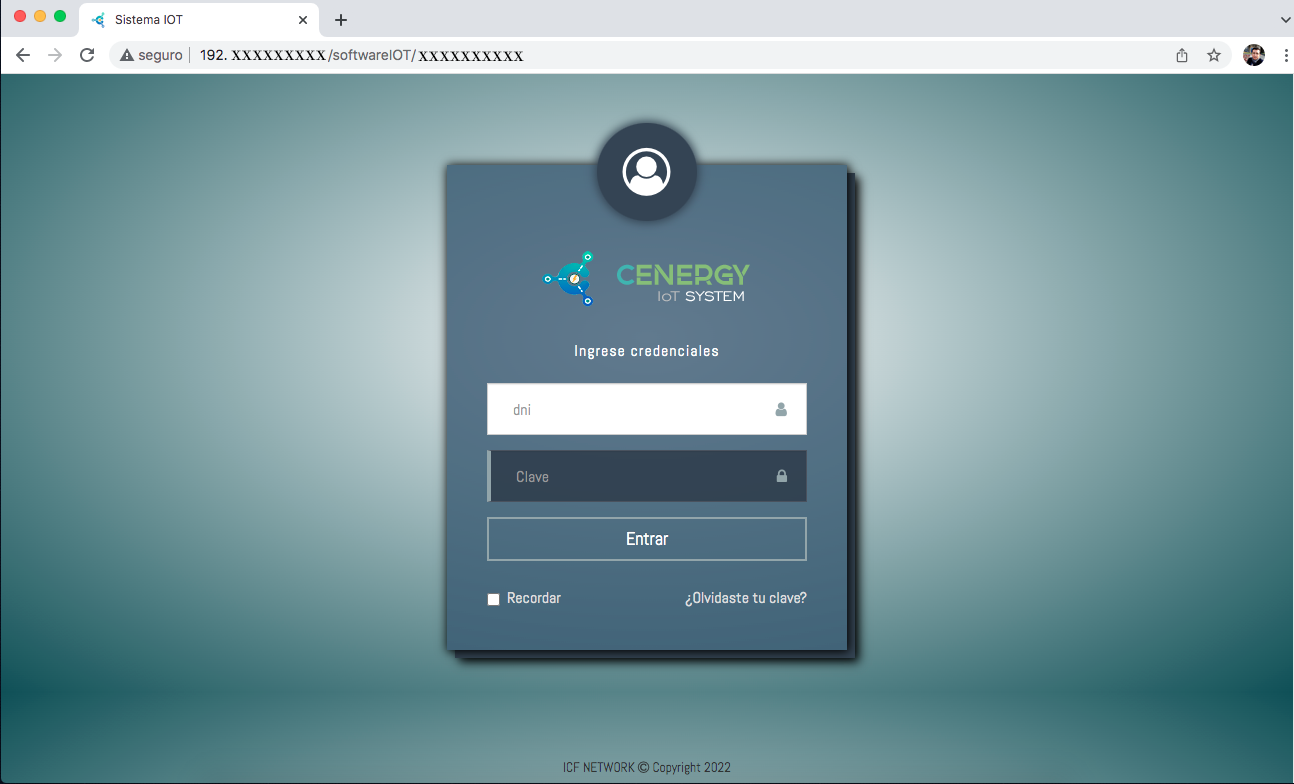
\includegraphics[width=1.55\textwidth]{./Figures/gui/0.png}
\caption{Interfaz gráfica de usuario de acceso al software de monitoreo y control.}
\label{fig:gui0}
\end{figure}
\end{landscape} %

%%%%%%%%%%%%%%%%%%%%%%%%%%%%%%%%%%%%%%%%%%%%%%%%%%%

%%%%%%%%%%%%%%%%%%%%%%%%%%%%%%%%%%%%%%%%%%%%%%%%%%%
\begin{landscape} % esto es para rotar la pagina e imagen
\begin{figure}[htpb]
\centering 
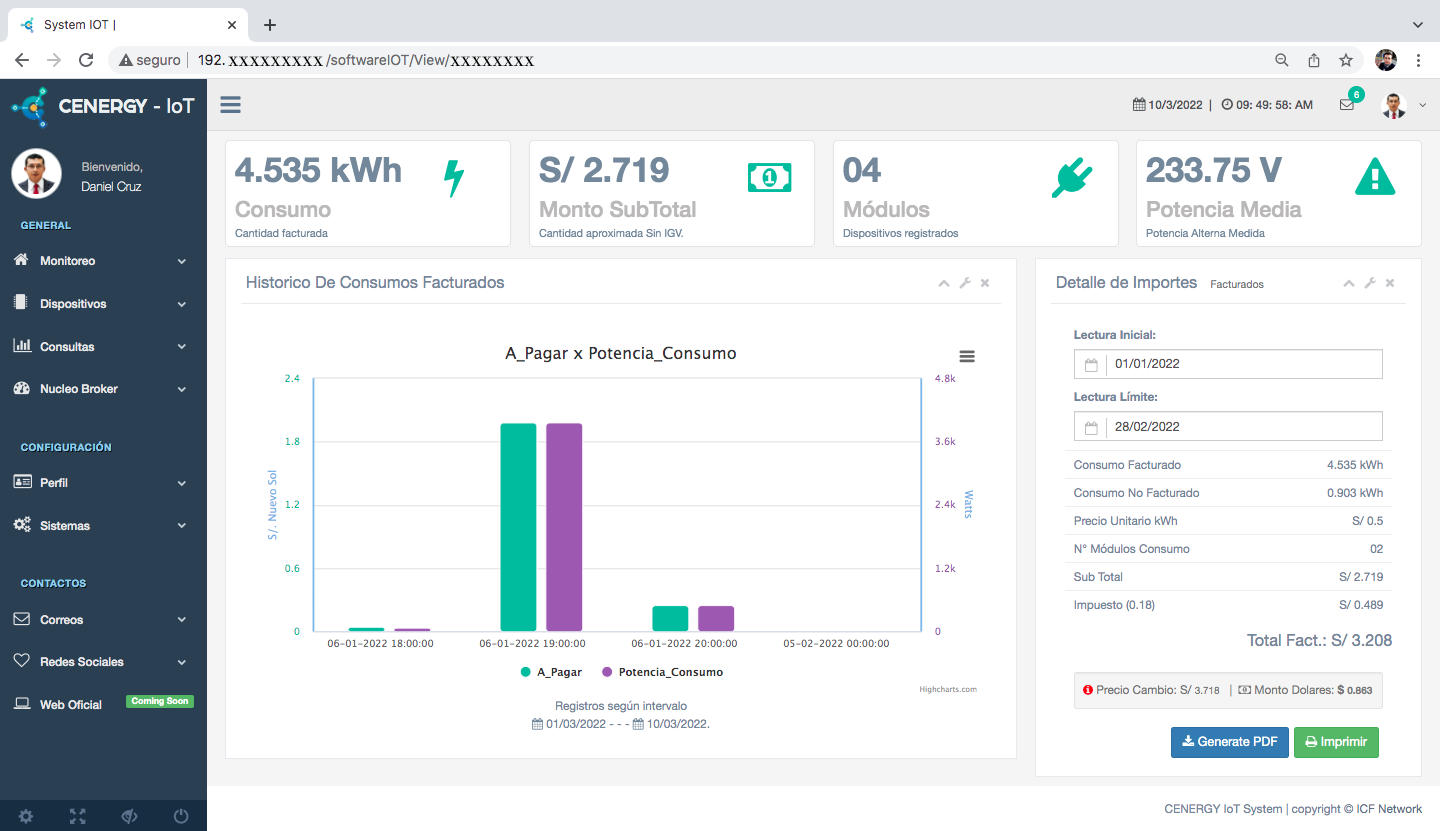
\includegraphics[width=1.55\textwidth]{./Figures/gui/1.png}
\caption{Dashboard inicial del software de monitoreo y control.}
\label{fig:gui1}
\end{figure}
\end{landscape} %

%%%%%%%%%%%%%%%%%%%%%%%%%%%%%%%%%%%%%%%%%%%%%%%%%%%

%%%%%%%%%%%%%%%%%%%%%%%%%%%%%%%%%%%%%%%%%%%%%%%%%%%
\begin{landscape} % esto es para rotar la pagina e imagen
\begin{figure}[htpb]
\centering 
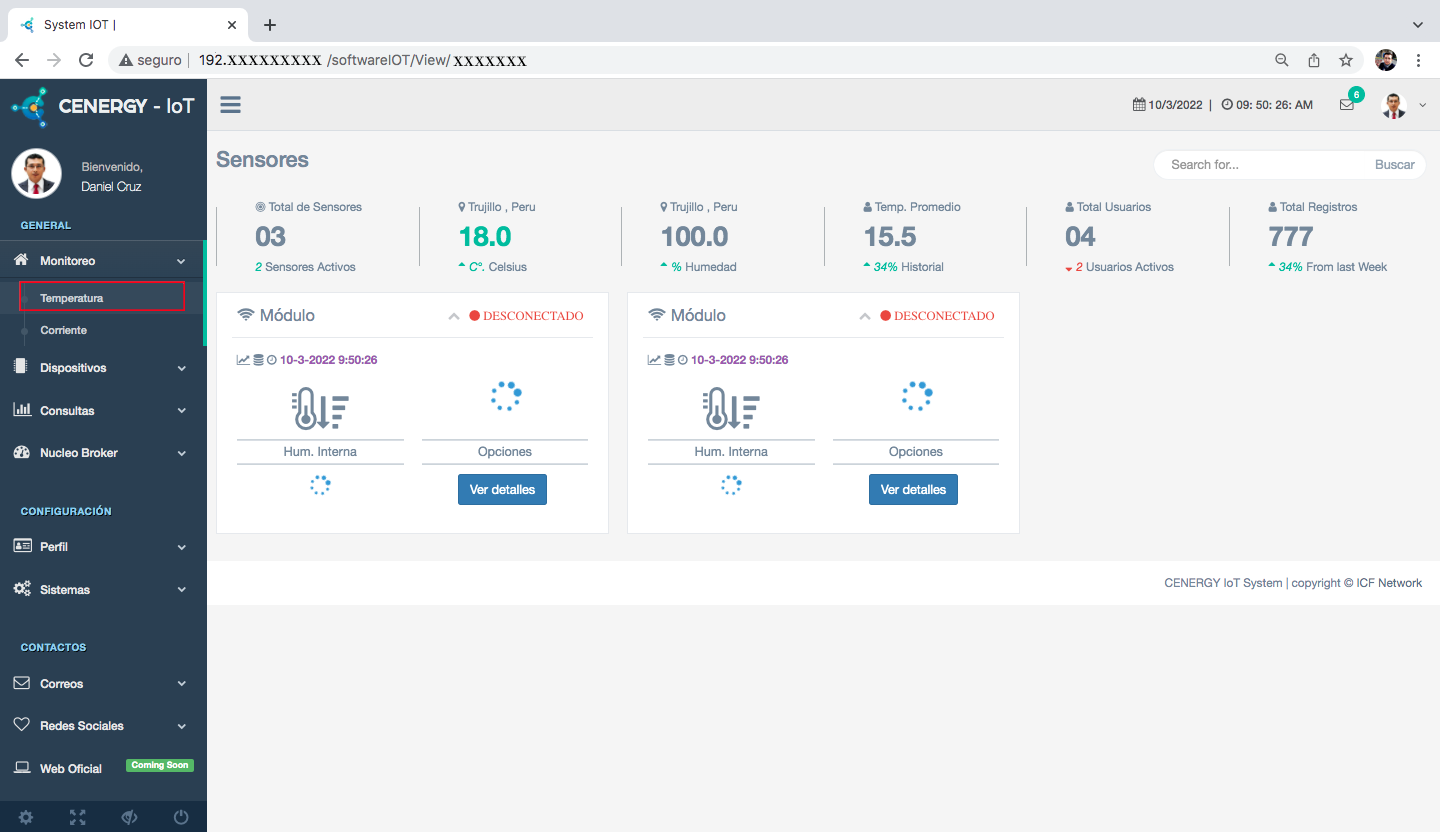
\includegraphics[width=1.55\textwidth]{./Figures/gui/2.png}
\caption{Interfaz gráfica de usuario donde se listan los sensores del sistema.}
\label{fig:gui2}
\end{figure}
\end{landscape} %

%%%%%%%%%%%%%%%%%%%%%%%%%%%%%%%%%%%%%%%%%%%%%%%%%%%

%%%%%%%%%%%%%%%%%%%%%%%%%%%%%%%%%%%%%%%%%%%%%%%%%%%
\begin{landscape} % esto es para rotar la pagina e imagen
\begin{figure}[htpb]
\centering 
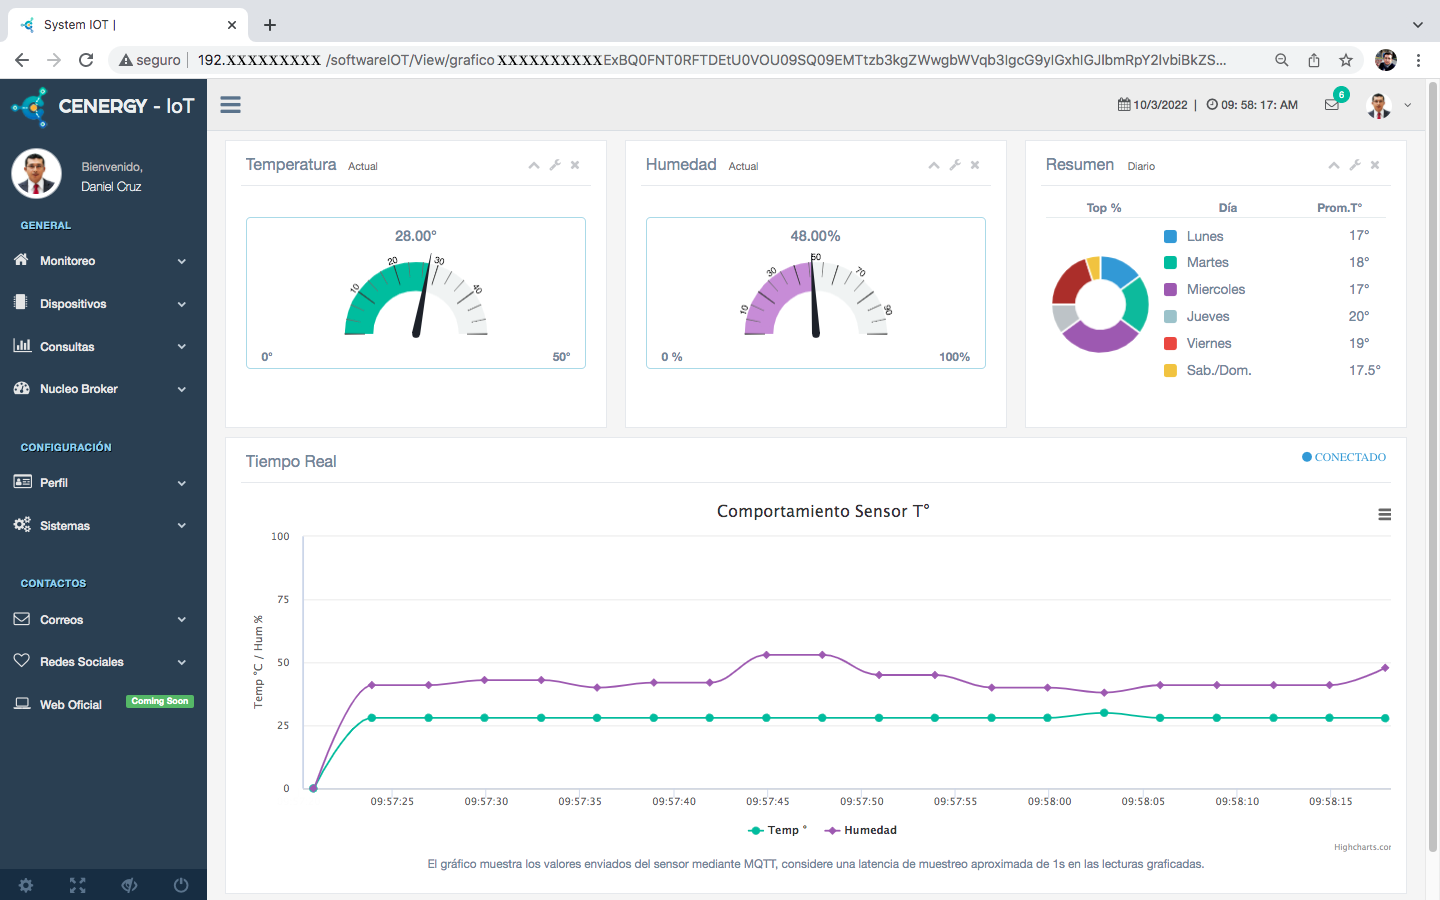
\includegraphics[width=1.5\textwidth]{./Figures/gui/2-1.png}
\caption{Interfaz gráfica de usuario donde se muestran todos los detalles de un sensor.}
\label{fig:gui2-1}
\end{figure}
\end{landscape} %

%%%%%%%%%%%%%%%%%%%%%%%%%%%%%%%%%%%%%%%%%%%%%%%%%%%

%%%%%%%%%%%%%%%%%%%%%%%%%%%%%%%%%%%%%%%%%%%%%%%%%%%
\begin{landscape} % esto es para rotar la pagina e imagen
\begin{figure}[htpb]
\centering 
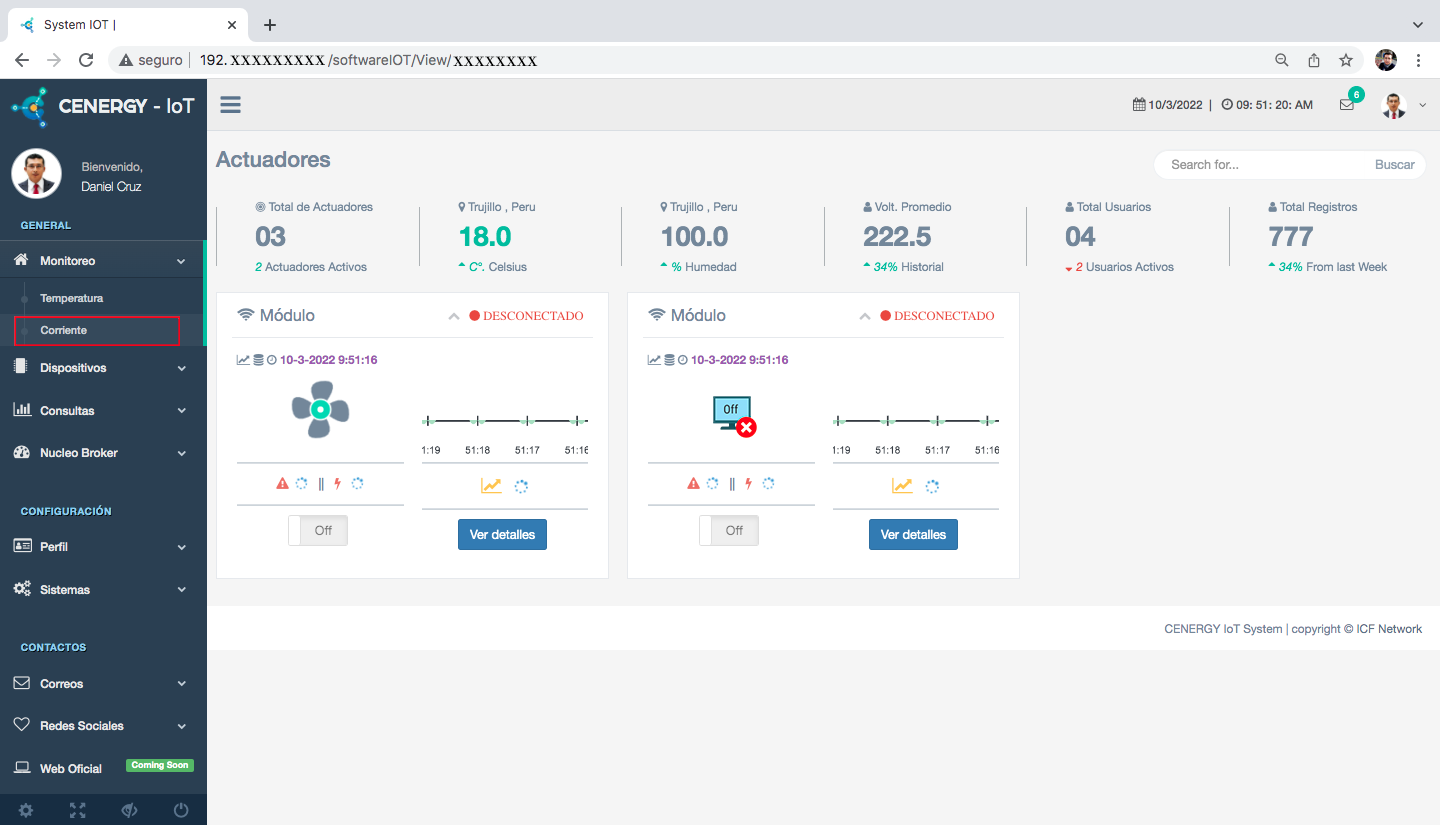
\includegraphics[width=1.52\textwidth]{./Figures/gui/3.png}
\caption{Interfaz gráfica de usuario donde se listan los sensores de consumo junto a su función de actuador.}
\label{fig:gui3}
\end{figure}
\end{landscape} %

%%%%%%%%%%%%%%%%%%%%%%%%%%%%%%%%%%%%%%%%%%%%%%%%%%%

%%%%%%%%%%%%%%%%%%%%%%%%%%%%%%%%%%%%%%%%%%%%%%%%%%%
\begin{landscape} % esto es para rotar la pagina e imagen
\begin{figure}[htpb]
\centering 
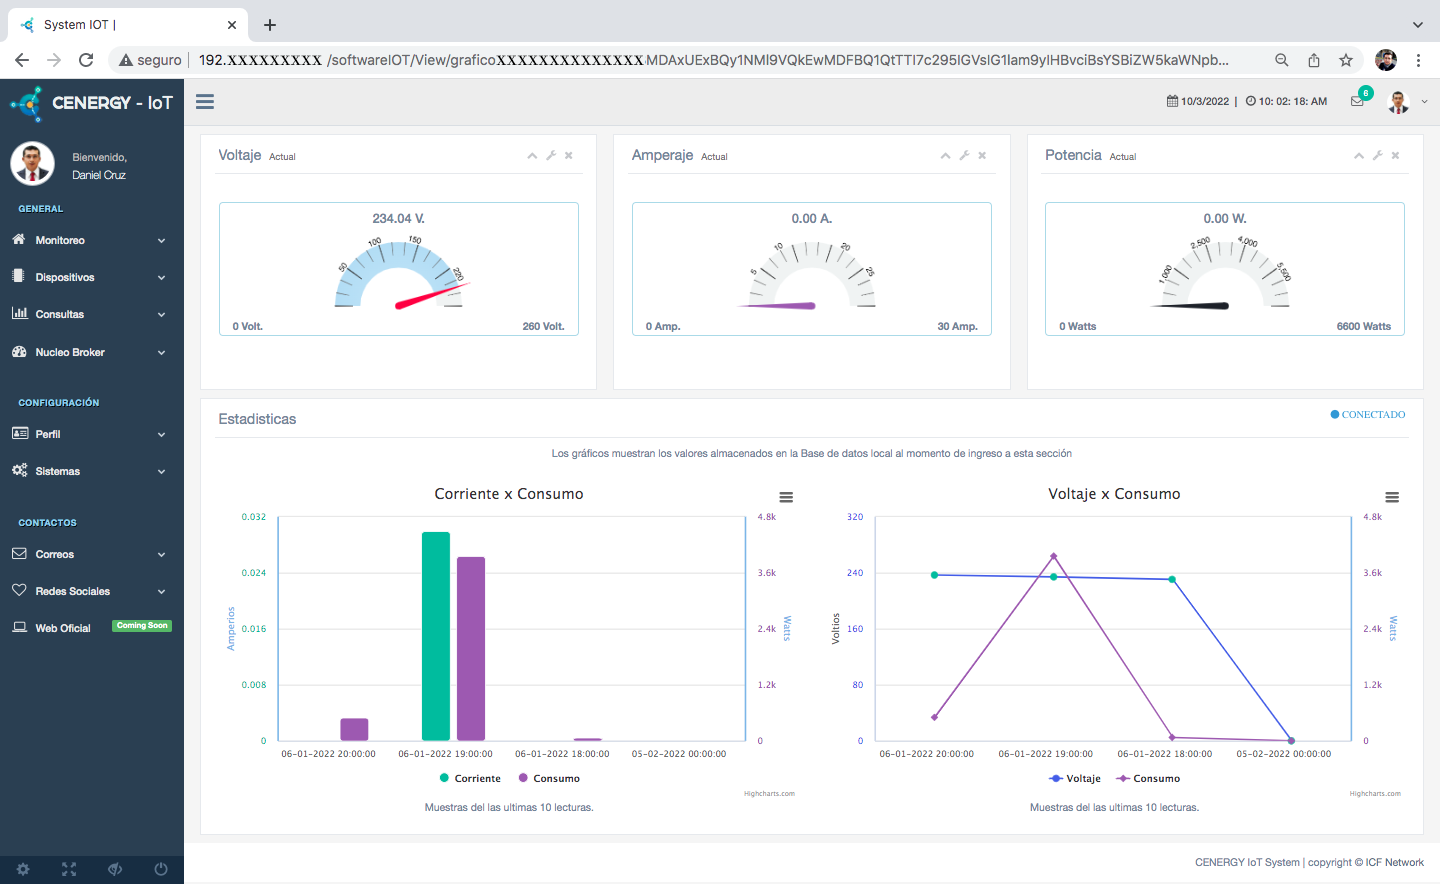
\includegraphics[width=1.52\textwidth]{./Figures/gui/3-1.png}
\caption{Interfaz gráfica de usuario donde se muestran todos los detalles de un sensor de consumo.}
\label{fig:gui3-1}
\end{figure}
\end{landscape} %

%%%%%%%%%%%%%%%%%%%%%%%%%%%%%%%%%%%%%%%%%%%%%%%%%%%

%%%%%%%%%%%%%%%%%%%%%%%%%%%%%%%%%%%%%%%%%%%%%%%%%%%
\begin{landscape} % esto es para rotar la pagina e imagen
\begin{figure}[htpb]
\centering 
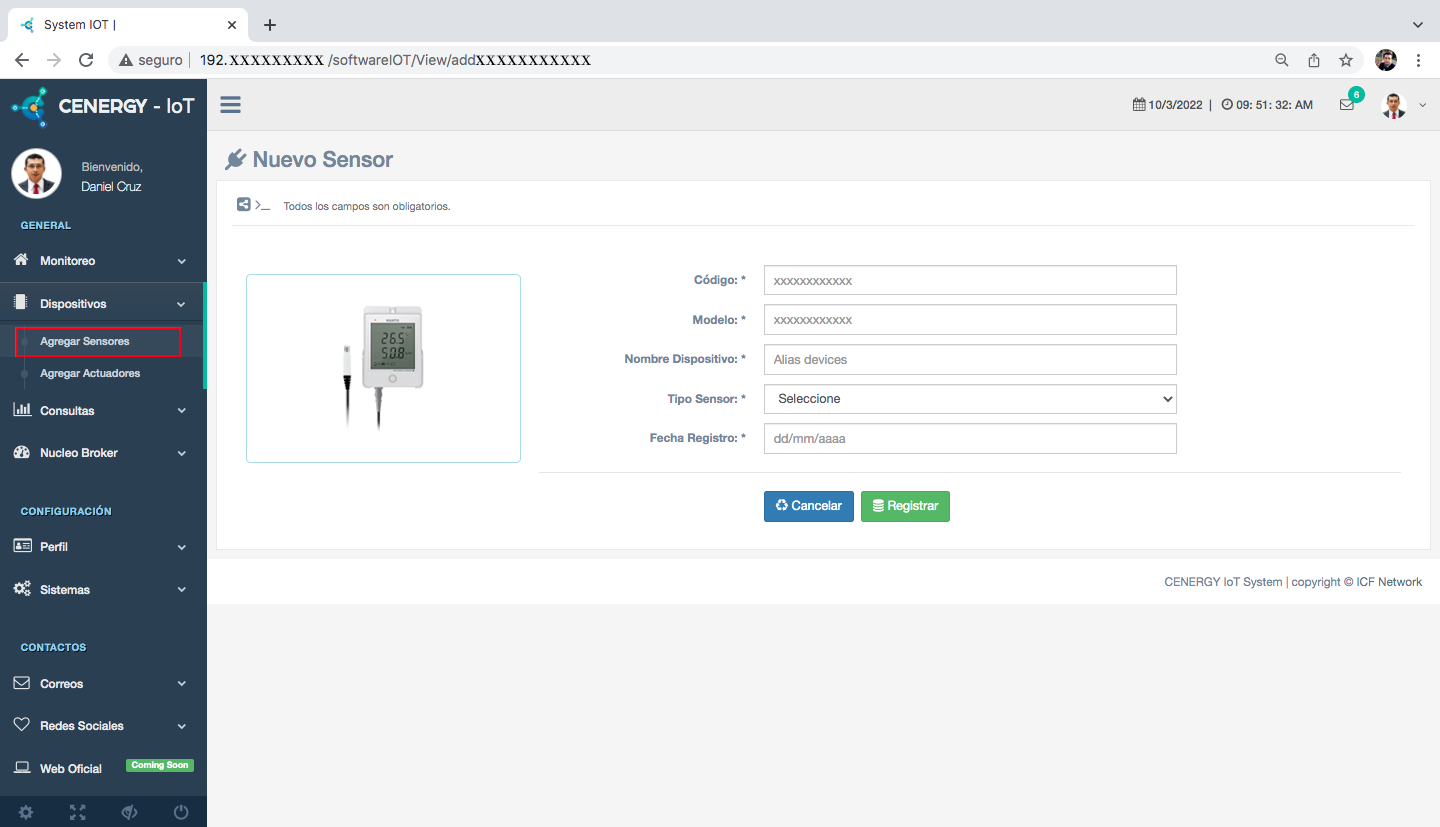
\includegraphics[width=1.55\textwidth]{./Figures/gui/4.png}
\caption{Interfaz gráfica de usuario para agregar un nuevo dispositivo al sistema.}
\label{fig:gui4}
\end{figure}
\end{landscape} %

%%%%%%%%%%%%%%%%%%%%%%%%%%%%%%%%%%%%%%%%%%%%%%%%%%%

%%%%%%%%%%%%%%%%%%%%%%%%%%%%%%%%%%%%%%%%%%%%%%%%%%%
\begin{landscape} % esto es para rotar la pagina e imagen
\begin{figure}[htpb]
\centering 
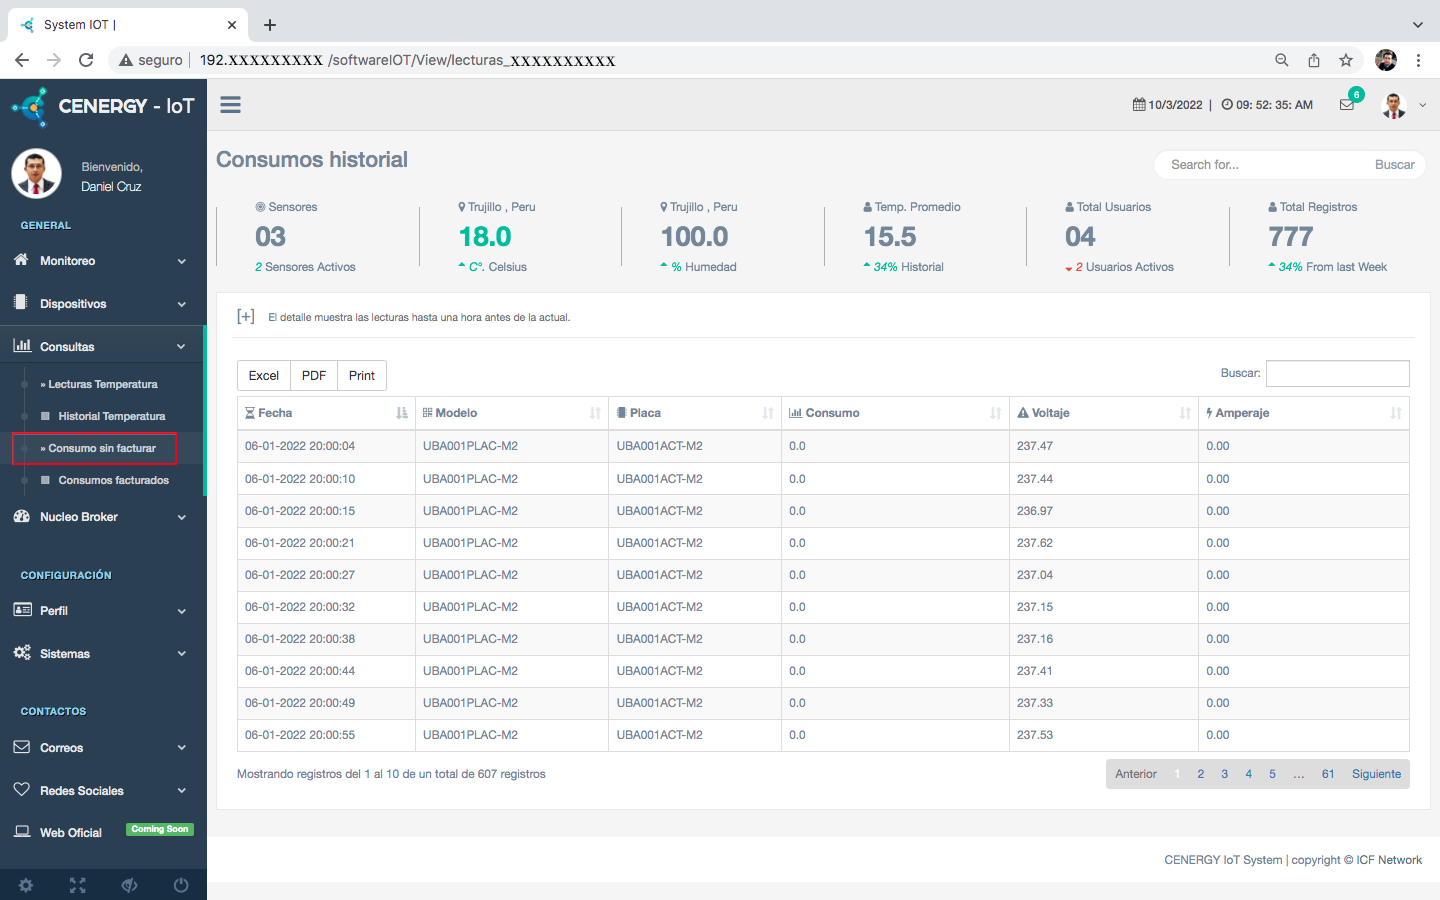
\includegraphics[width=1.5\textwidth]{./Figures/gui/5.png}
\caption{Interfaz gráfica de usuario donde se muestran las consultas y reportes de la base de datos.}
\label{fig:gui5}
\end{figure}
\end{landscape} %

%%%%%%%%%%%%%%%%%%%%%%%%%%%%%%%%%%%%%%%%%%%%%%%%%%%

\section{Pruebas de elección de canal y ancho de banda}


Los fundamentos y consideraciones para la mejoren la elección del canal y ancho de bana del canal Wi-Fi IoT que se utilizó se describió en el ....capitulo 3 .... La elección dependió de las señales circundantes vecinas a la red domestica donde se instaló el sistema prototipo IoT. La figura.... muestra resultado del primer escaneo de las señales y el uso de los canales respectivos así como solapamiento existente entre ellos. 

De la imagen se describe lo siguiente:

\keyword{Señal WLAN IoT} 
\begin{itemize}
\item SSID: MATRIX-ICF
\item Canal: 10 (configuración automática)
\item Ancho de canal: 40 MHz (configuración automática)
\item Potencia señal: 93\%
\item Seguridad:  WPA2 (PSK)
\item Tasa Máxima de transferencia: 300 Mbps
\end{itemize}


\keyword{Señal WLAN doméstica}
\begin{itemize} 
\item SSID: CLARO-B612-D514
\item Canal: 11 (configuración automática)
\item Ancho de canal: 20 MHz (configuración automática)
\item Potencia señal: 64\%
\item Seguridad: WPA2 (PSK)
\item Tasa Máxima de transferencia: 144.4 Mbps
\end{itemize}

El procedimiento de mejora consistió en modificar la configuración por defecto del router/AP de la red IoT al cambiar el canal y reducir el ancho de banda, verificando en cada cambio el comportamiento de las señales en el ambiente y la reducción de solapamiento de los mismos.

%%%%%%%%%%%%%%%%%%%%%%%%%%%%%%%%%%%%%%%%%%%%%%%%%%%
\begin{landscape} % esto es para rotar la pagina e imagen
\begin{figure}[htpb]
\centering 
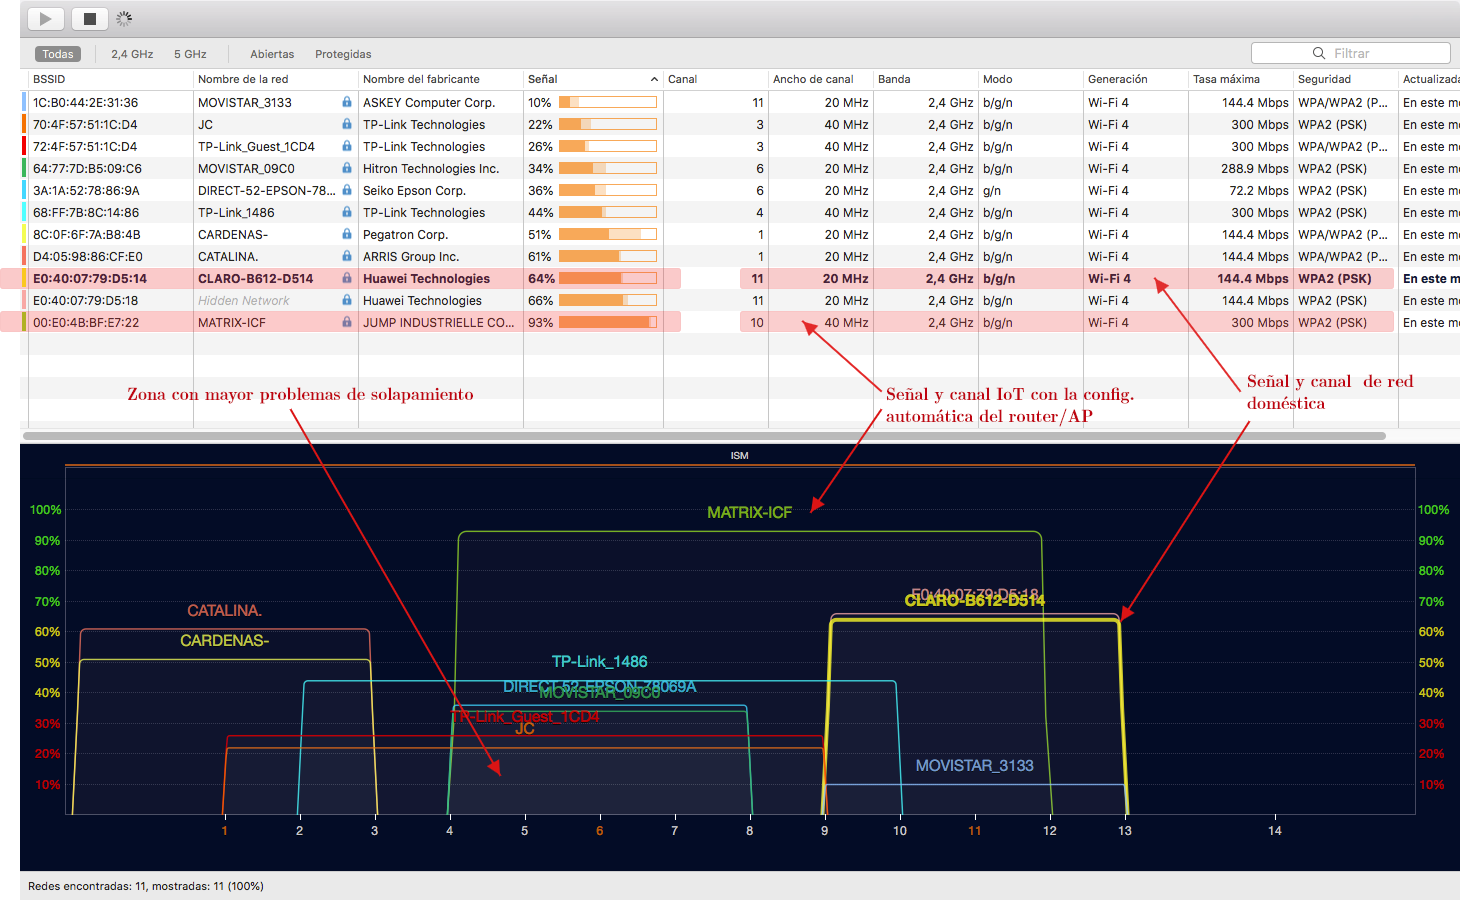
\includegraphics[width=1.5\textwidth]{./Figures/wifi/01.png}
\caption{..... .}
\label{fig:test01}
\end{figure}
\end{landscape} %

%%%%%%%%%%%%%%%%%%%%%%%%%%%%%%%%%%%%%%%%%%%%%%%%%%%

\begin{landscape} % esto es para rotar la pagina e imagen
\begin{figure}[htpb]
\centering 
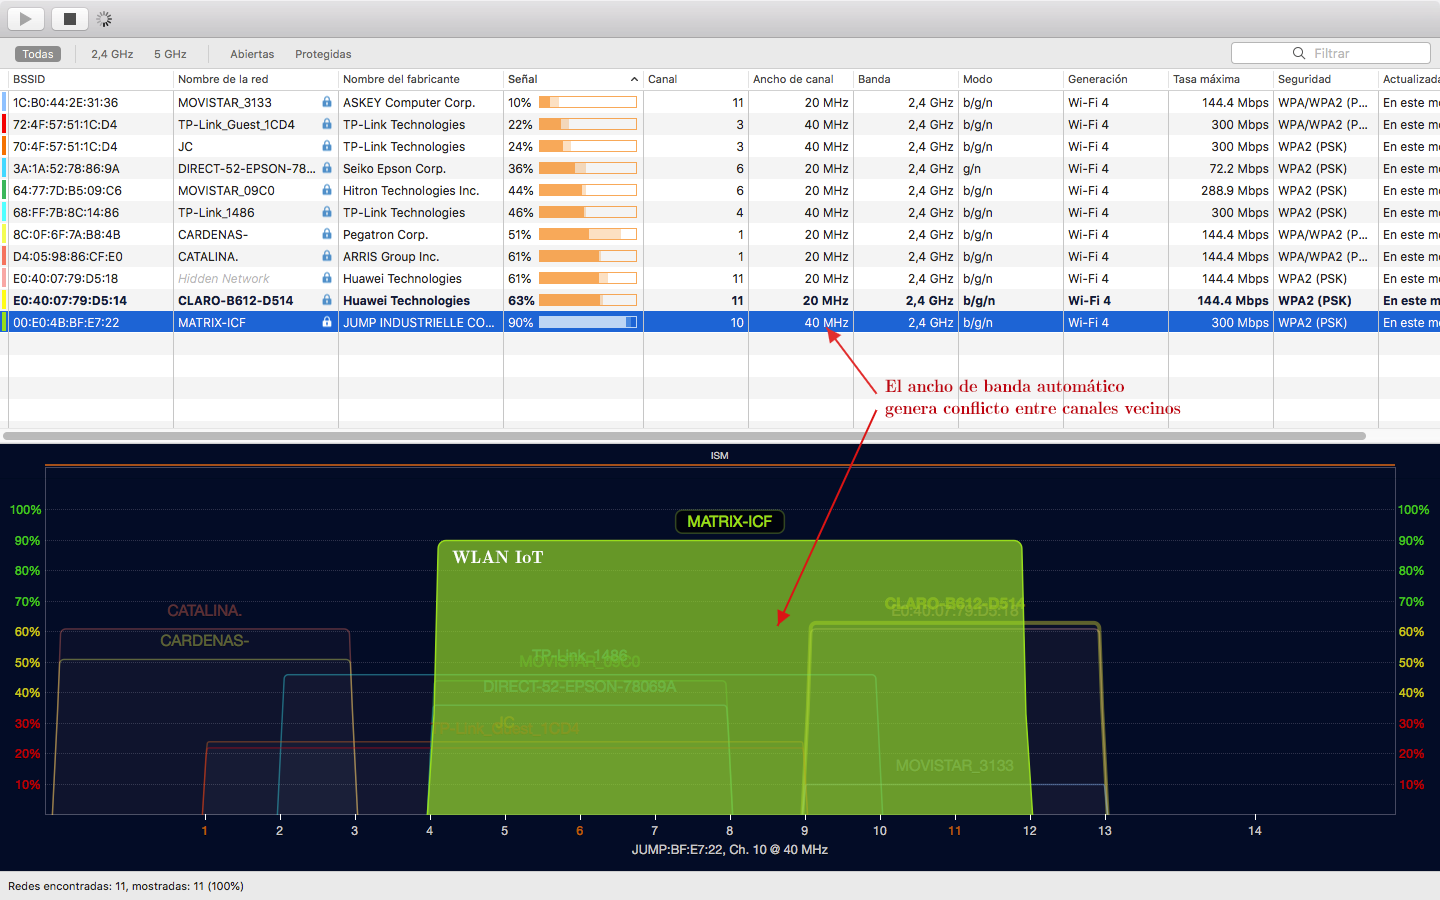
\includegraphics[width=1.5\textwidth]{./Figures/wifi/02.png}
\caption{..... .}
\label{fig:test02}
\end{figure}
\end{landscape} %


%%%%%%%%%%%%%%%%%%%%%%%%%%%%%%%%%%%%%%%%%%%%%%%%%%%
\begin{landscape} % esto es para rotar la pagina e imagen
\begin{figure}[htpb]
\centering 
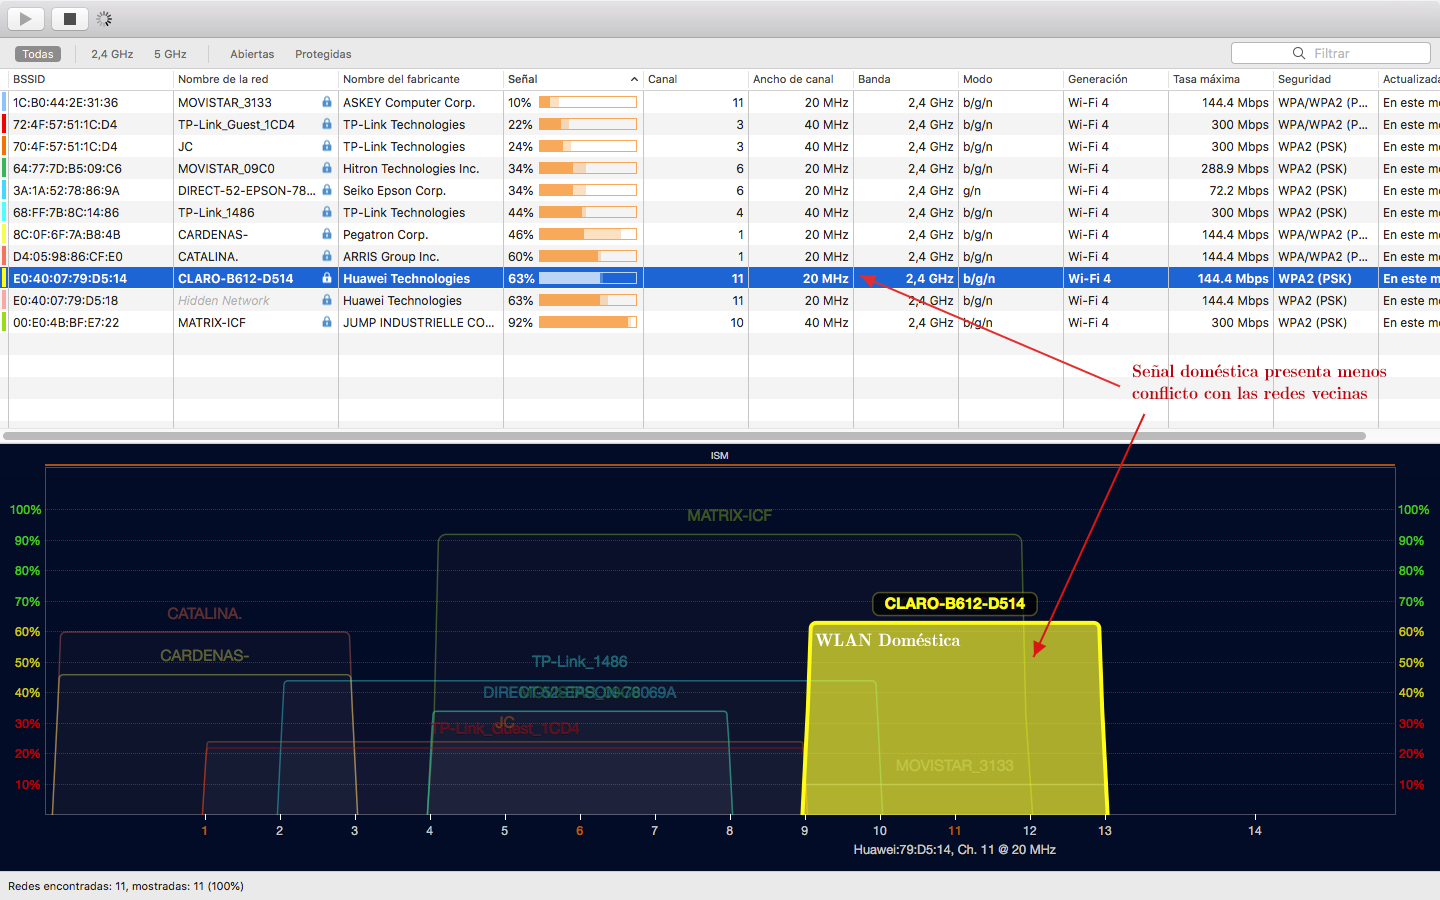
\includegraphics[width=1.5\textwidth]{./Figures/wifi/03.png}
\caption{..... .}
\label{fig:test03}
\end{figure}
\end{landscape} %

%%%%%%%%%%%%%%%%%%%%%%%%%%%%%%%%%%%%%%%%%%%%%%%%%%%

\begin{landscape} % esto es para rotar la pagina e imagen
\begin{figure}[htpb]
\centering 
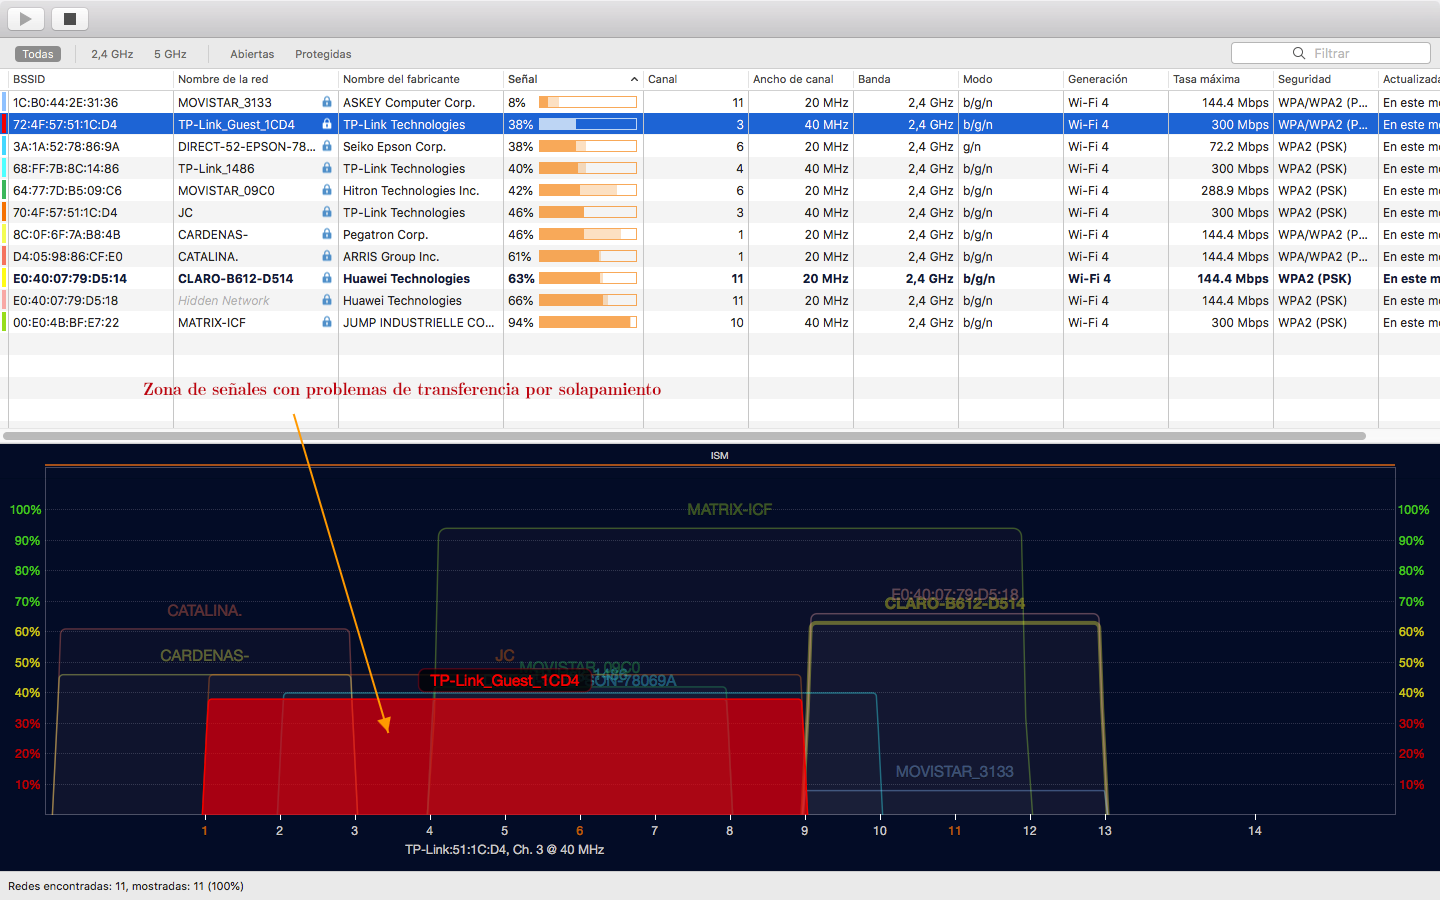
\includegraphics[width=1.5\textwidth]{./Figures/wifi/04.png}
\caption{..... .}
\label{fig:test04}
\end{figure}
\end{landscape} %


%%%%%%%%%%%%%%%%%%%%%%%%%%%%%%%%%%%%%%%%%%%%%%%%%%%

\begin{landscape} % esto es para rotar la pagina e imagen
\begin{figure}[htpb]
\centering 
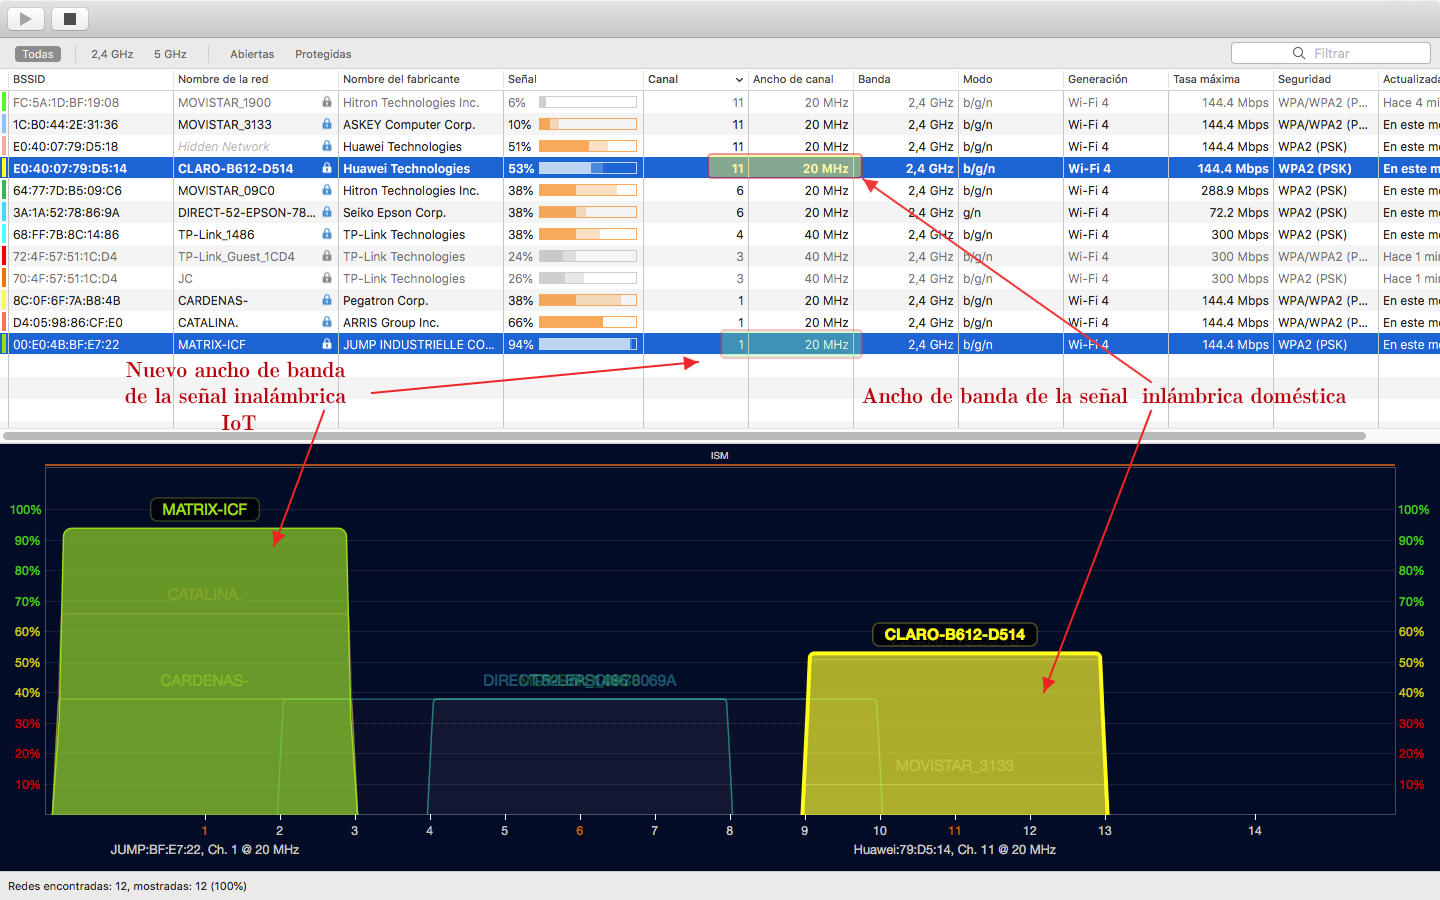
\includegraphics[width=1.5\textwidth]{./Figures/wifi/05.png}
\caption{..... .}
\label{fig:test05}
\end{figure}
\end{landscape} %


%%%%%%%%%%%%%%%%%%%%%%%%%%%%%%%%%%%%%%%%%%%%%%%%%%%

\begin{landscape} % esto es para rotar la pagina e imagen
\begin{figure}[htpb]
\centering 
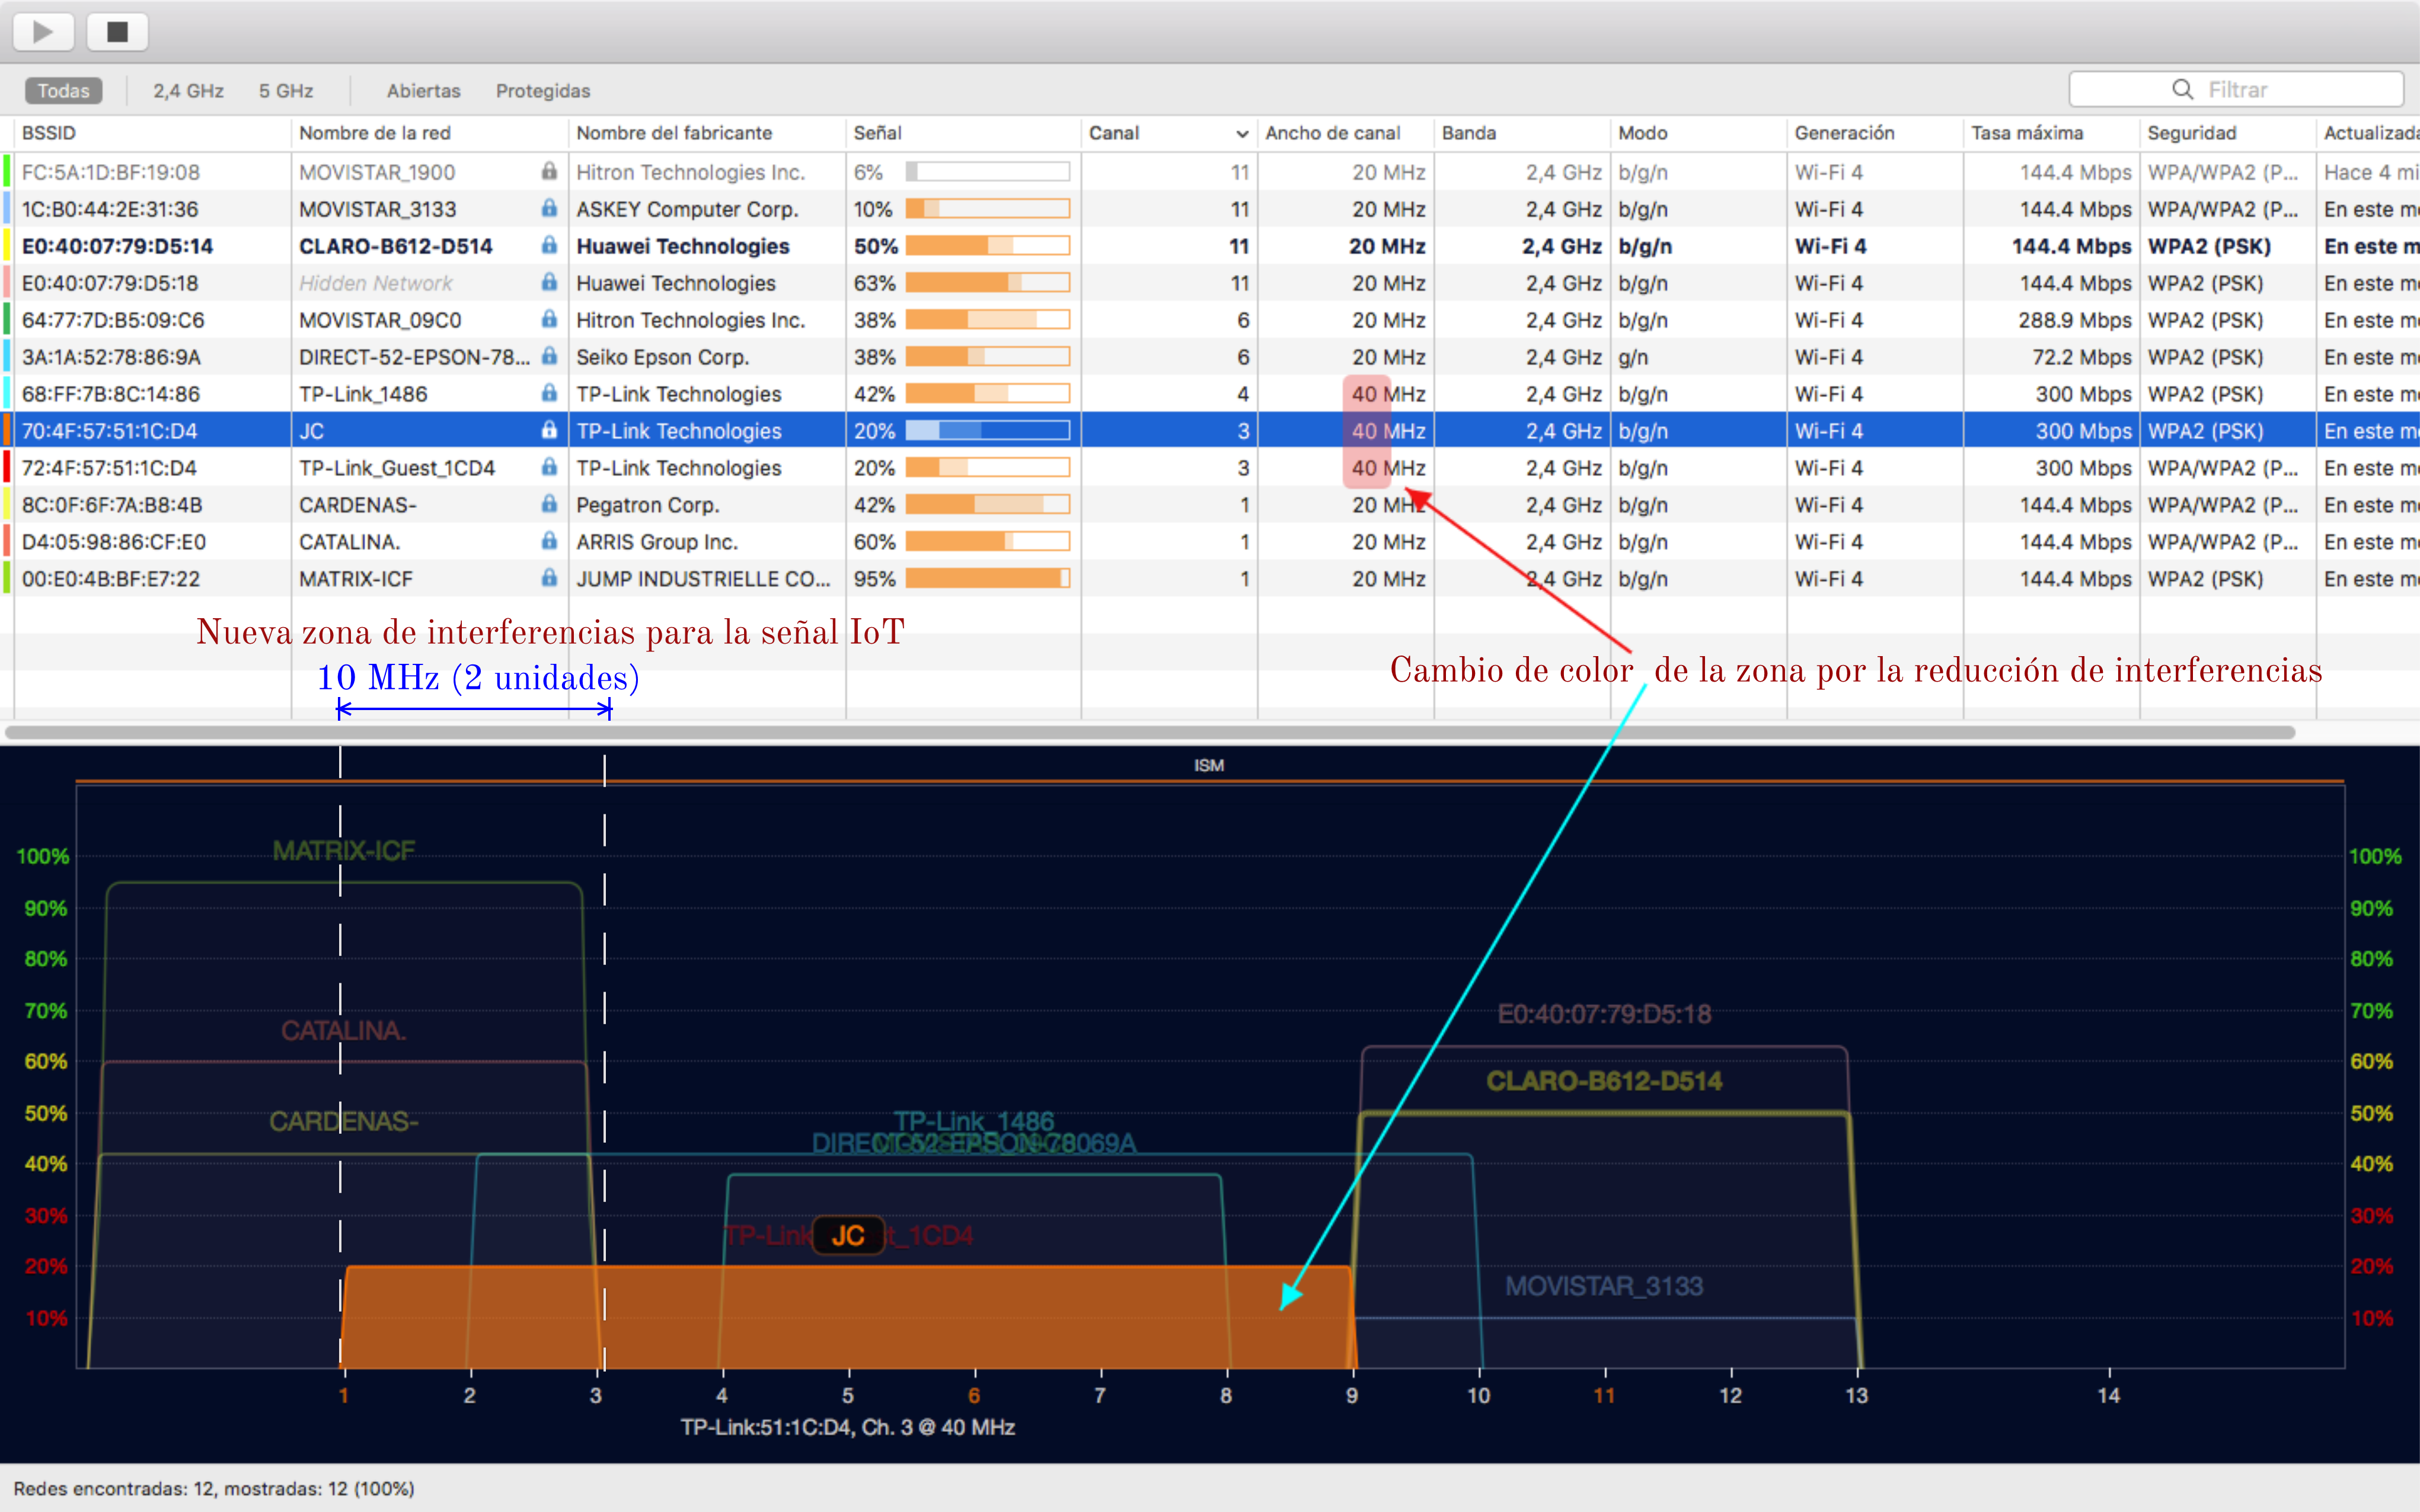
\includegraphics[width=1.5\textwidth]{./Figures/wifi/06.png}
\caption{..... .}
\label{fig:test06}
\end{figure}
\end{landscape} %


\section{Pruebas del módulo de temperatura}
\section{Pruebas del módulo actuador y consumo}
\section{Pruebas del funcionamiento del módulo replicador}
\section{Pruebas del funcionamiento del sistema sin Internet}
\section{Pruebas y resultados de consumo de energía eléctrica}
\section{Pruebas funcionales del sistema desde acceso remoto}
